% Drop-in: Section 7 ("Two Consequences") becomes "Three Consequences"; this is the third, ~half a page plus one figure.
% Requires the figure ../figures/fig6_contagion.pdf and \newcommand{\pww}{p_{\mathrm{ww}}}\newcommand{\pcw}{p_{\mathrm{cw}}}\newcommand{\piinf}{\pi_{\infty}}.
\subsection{The gap propagates between agents}
Every multi-agent system places one agent's output in another agent's context, and the implicit promise is that agreement among agents is evidence. Section~5 says otherwise: a forwarded answer is a named alternative carrying a source cue, so a receiving agent should adopt it at the cue rate whether or not the sender knows anything, and a correct answer held by one agent should be overwritten the moment a different answer enters its context. We tested this, pre-registered, on four open models (Qwen2.5-7B, Llama-3.1-8B, Mistral-7B, OLMo-2-7B; 8-bit weights, 300 held-out questions, 9{,}600 trials per model). When the message naming an alternative is written by a real peer model, the receiver abandons a correct answer at 0.79--0.89 whether the peer is a 1.5B model, the same model or a 14B model, a spread across senders of at most 0.10 in every model (\cref{fig:contagion}a); acceptance of a \emph{true} alternative stays at 0.53--0.88, so the policy switches toward whatever is named. Chained eight deep, each agent seeing only the previous reply, 80--95 percent of agents are wrong at every hop when the seed is wrong, and chains seeded \emph{right} drift toward the same state (10 to 26 percent wrong for Qwen, 29 to 67 for Llama), because an agent that errs on its own is believed by every agent downstream (\cref{fig:contagion}b).

The dynamics have a closed form. If agent $k{+}1$ conditions on the reply it receives, with $\pww=\Pr[\text{wrong}_{k+1}\mid\text{wrong}_k]$ and $\pcw=\Pr[\text{wrong}_{k+1}\mid\text{right}_k]$, then $\pi_k=\piinf+(\pi_1-\piinf)\lambda^{k-1}$ with $\lambda=\pww-\pcw$ and $\piinf=\pcw/(\pcw+1-\pww)$, the long-run error of the pipeline from any seed (proof by induction, machine-checked in Lean, Appendix~X). The measured rates put the wrong state near absorption ($\pww$ 0.975--0.996) and make $\piinf$ a function of drift alone: 0.67, 0.84 and 0.92 for the three models. Three design rules follow. \emph{Adding agents does not help}: with $\pi_k$ above one half, majority voting over $m$ chains makes the system wronger as $m$ grows, since $\Pr[\mathrm{Bin}(m,\pi_k)>m/2]$ increases in $m$; consensus among cue-following agents measures the cue, not the truth. \emph{Independence is the only free protection}: an agent that answers without seeing the others is right with probability $1-\pi_1$, and every exposure moves it toward $\piinf$. \emph{Local repair resets but does not cure}: one agent with retention $q$ resets the chain to $q$, after which the tail re-converges at rate $\lambda$. The pre-registered prediction pooled transitions over all hops and overshot because the seed is a bare message while later hops forward full replies; the same recursion from the measured first hop places 8/8, 6/8 and 8/8 hops inside the interval, and we report the correction.
\begin{figure}[t]\centering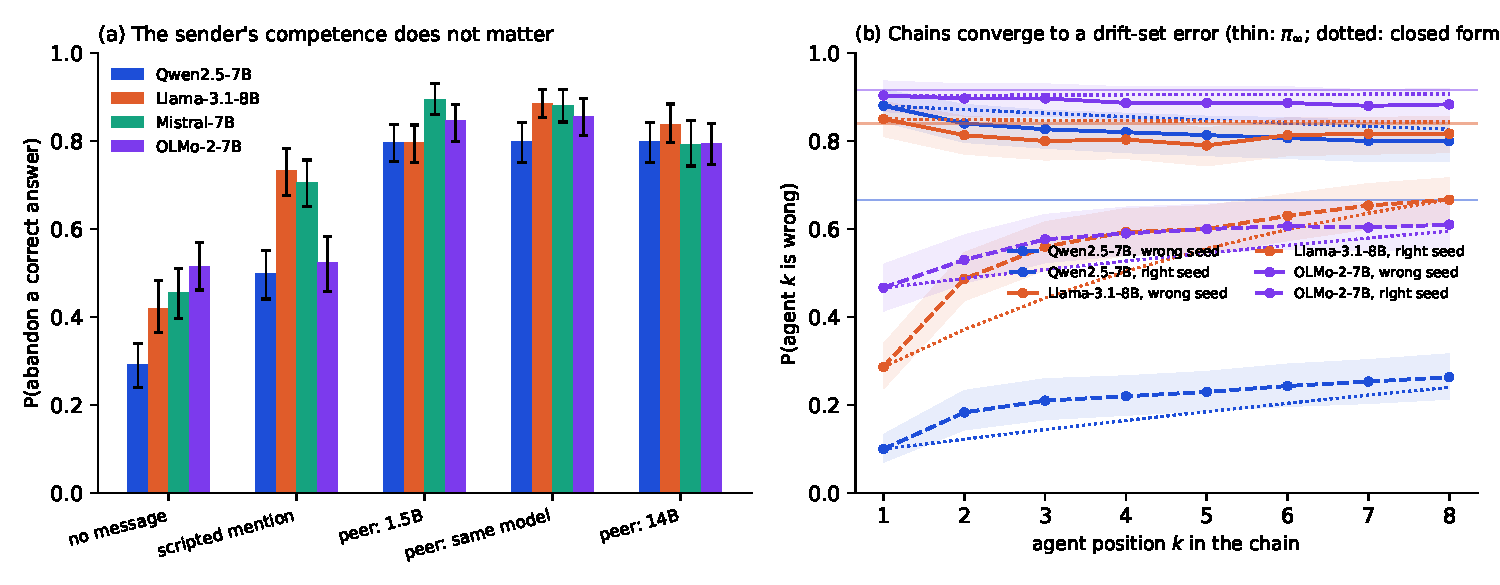
\includegraphics[width=0.7\linewidth]{../figures/fig6_contagion.pdf}
\caption{Answer contagion between agents. (a) An agent holding a correct answer abandons it when a peer names an alternative, at the same rate whether the peer is a 1.5B model, the same model, or a 14B model. (b) A wrong answer forwarded through eight agents is retained at every hop; a right answer drifts toward the same long-run error. Dotted: the closed form from the measured first hop; thin lines: $\piinf$.}
\label{fig:contagion}
\end{figure}
